\chapter{Frameworks}
\section{Introduction to Machine Learning}

Machine learning is a powerful tool that can be used to identify patterns in complex datasets. In the context of particle physics, machine learning algorithms can be used to detect signals from background noise in large datasets generated by detectors. In particular, for the detection of IBD signals from background, machine learning algorithms can be used to identify patterns in the data that are indicative of an IBD event, and to distinguish these signals from the background noise explained above. Moreover, one advantage of machine learning for particle physics is that it can handle large amounts of data and identify subtle patterns that may be difficult for humans to detect.
\\


\subsection{Supervised Learning}

Supervised learning is a machine learning technique in which the algorithm is trained on a labelled dataset, where the input data is accompanied by the correct output. The goal of the algorithm is to learn a function that can map input data to output data. Some examples of supervised learning algorithms include linear regression, logistic regression, decision trees, and support vector machines. Despite the complexity and diversity of these methods, it's more advantageous to illustrate the profound concepts of machine learning through a simple machine learning algorithm, such as linear regression. 

\subsection{Linear Regression}
Linear regression is a type of supervised learning algorithm used in machine learning for predictive analysis. It is used to model the relationship between a dependent variable, called the target, and one or more independent variables, called the features.
\\
The basic idea behind linear regression is to find the best-fitting hyper-plane that describes the relationship between the independent and dependent variables. The equation for the hyper-plane can be written as:

\begin{equation}
	y = w_0 + w_1 x_1 + w_2 x_2 + ... + w_n x_n 
\end{equation}
 where 
\begin{itemize}
	\item $y$ is the dependent variable
	\item $x_1, x_2, ..., x_p$ are the independent variables
	\item $w_0, w_1, w_2, ..., w_n$ are the coefficients or parameters of the model
\end{itemize}

In order to determine the values of the coefficients $w_0, w_1, w_2, ..., w_n$, a common approach is to minimize a loss function, which measures the difference between the predicted values of the dependent variable and the actual values. The most commonly used loss function in linear regression is the mean squared error (MSE) function, which is defined as:

\begin{equation}
	L(w_0, w_1, w_2, ..., w_n) = \frac{1}{n} \sum_{i=1}^{n} (y_i - \hat{y_i})^2
\end{equation}

where $n$ is the number of observations, $y_i$ is the actual value of the dependent variable for the $i$-th observation, and $\hat{y_i}$ is the predicted value of the dependent variable for the $i$-th observation.


The objective of linear regression is to determine the optimal values of coefficients $w_0, w_1, w_2, ..., w_n$ that minimize a predefined loss function $L(w_0, w_1, w_2, ..., w_n)$. One commonly employed method to accomplish this is the gradient descent algorithm.\\


Gradient descent is an iterative optimization technique for finding the local minimum of a function. To apply gradient descent in the context of a linear regression problem, we initialize the coefficients with random values and then iteratively update these values in the direction that decreases the loss function the most.

Mathematically, the update rule for each coefficient is:

\begin{equation}
	w_j^{(new)} = w_j^{(old)} - \alpha \frac{\partial L}{\partial w_j}
\end{equation}


where $w_j^{(new)}$ and $w_j^{(old)}$ are the new and old values of the j-th coefficient, $\alpha$ is the learning rate, and $\frac{\partial L}{\partial w_j}$ is the partial derivative of the loss function with respect to the j-th coefficient. The learning rate $\alpha$ determines the size of the steps we take towards the minimum.

Once we reach a point where the loss function no longer decreases (or decreases very slowly), we stop the iteration and accept the current values of coefficients as the solution.
\\

However, it is important to note that linear regression, and also other machine learning alghoritms can suffer from overfitting or underfitting. Overfitting occurs when the model is too complex and captures noise in the data, while underfitting occurs when the model is too simple and fails to capture the underlying patterns in the data. To prevent overfitting or underfitting, regularization techniques can be used.

\newpage

\section{Binary Classification}
The binary classification problem is a fundamental task in supervised learning, a branch of machine learning. It involves classifying elements of a dataset into one of two possible groups based on a set of features. For instance, a binary classification problem could involve determining whether an email is spam or not spam, whether a transaction is fraudulent or legitimate, or whether a tumor is malignant or benign.

To tackle the binary classification problem, various machine learning algorithms can be employed. Two common approaches are \textit{Decision Trees} and \textit{Neural Networks}. 

\section{Decision Tree}
A Decision Tree algorithm, used in supervised machine learning for classification and regression tasks, models the predictive outcome of a target variable based on decision rules inferred from input features. The process involves dissecting the overall dataset into distinct regions, where each region contains data points that are as similar as possible to each other in terms of their target class. Formally, each internal node of the tree represents a decision rule based on an input feature, which bifurcates the data into two child nodes. The decision for splitting the data at each node is determined using a metric known as Information Gain, which in turn is based on the concept of Entropy.

In the context of a binary classification, entropy (H) is a measure of the impurity or disorder within a set (S) of instances. It quantifies the uncertainty involved in predicting the class of a random instance from the set (S). It is mathematically formulated as:

\begin{equation}
	H(S) = - p_{+} \log_{2}(p_{+}) - p_{-} \log_{2}(p_{-})
\end{equation}

Here, $p_+$ and $p_-$ denote the proportions of positive and negative instances in the set S, respectively. Entropy attains a maximum value when the set S contains an equal number of positive and negative instances, reflecting the highest uncertainty.

Information Gain (IG) measures the reduction in entropy achieved by partitioning the instances based on a feature (A). It is the difference between the entropy of the set before the split (H(S)) and the weighted sum of the entropies of each subset resulting from the split. It can be formulated as:

\begin{equation}
	IG(S, A) = H(S) - \sum_{v \in V(A)} \left(\frac{|S_v|}{|S|}\right) H(S_v)
\end{equation}

where $V(A)$ indicates the set of all possible values of feature A.\\
In this equation, $S_v$ denotes the subset of instances in S for which the feature A takes on the value v. $|S_v|$ and $|S|$ are the cardinalities of the sets $S_v$ and $S$, respectively.\\

The algorithm constructs the tree by recursively applying these splits, each time selecting the feature that results in the maximum information gain. This process continues until a stopping criterion is met, such as reaching a pre-specified maximum depth of the tree or a minimum number of samples per leaf.\\


While Decision Trees are straightforward and practical models, their ability to decipher complex patterns in data can be limited. This limitation paves the way for a more advanced technique known as Gradient Boosting Decision Trees. This innovative method combines several simple trees into a robust model that can effectively interpret intricate patterns in complex datasets. The following sections will delve into the mechanics of Gradient Boosting Decision Trees and their enhanced ability to handle complex data structures.

\subsection{Gradient Boosting Decision Trees}

 %[] https://www.youtube.com/watch?v=PxgVFp5a0E4&ab_channel=Prof.RyanAhmed
Gradient Boosting is a machine learning algorithm that stems from the concept of boosting, with the application of gradient descent methodology. Its goal is to produce a robust predictive model through the combination of multiple weak learners, typically decision trees.

The primary innovation in Gradient Boosting over classical boosting techniques is its approach to error correction. Instead of modifying the weights of misclassified instances, Gradient Boosting fits each new tree to the residuals (or the negative gradient) of the loss function with respect to the prediction of the existing ensemble of trees. This means each new tree is trained to predict the error of the existing model, thereby iteratively reducing the overall error.

Let's formalize this process:

\begin{enumerate}
	\item \textbf{Initialization}: We begin by initializing our model with a constant value. This is denoted as $F_0(x) = \arg\min_{\gamma} \sum_{i=1}^{N} L(y_i, \gamma)$, where $L(y, F(x))$ represents the loss function, $y$ represents the true target value, and $F(x)$ is the model's prediction for the input features $x$. This constant prediction, $\gamma$, is chosen to minimize the total loss over all $N$ instances. Thus, our initial model starts with a prediction that globally minimizes the loss.
	\item \textbf{Computation of Residuals}: Next, we iteratively construct an ensemble of $M$ trees. For each iteration $m=1$ to $M$, we calculate the residuals as
	\begin{equation}
		r_{im} = - \left[\frac{\partial L(y_i, F(x_i))}{\partial F(x_i)}\right]_{F(x)=F_{m-1}(x)}
	\end{equation} 
 	for each instance $i=1,2,...,N$. These residuals are essentially the negative gradients (or first derivatives) of the loss function with respect to the model's predictions. They provide a measure of the direction that would decrease the loss function fastest.
	\item \textbf{Fitting a Decision Tree}: After computing the residuals, we fit a new decision tree, $h_m(x)$, to these residuals. This tree is thus trained to predict the negative gradient of the loss function, using train it using the training set 
	${(x_i, r_{im})}_{i=1}^n$. By doing so, it attempts to correct the errors made by the current ensemble model.
	\item \textbf{Model Update}: The model is then updated by applying the rule
	\begin{equation}
		F_m(x) = F_{m-1}(x) + \nu \cdot h_m(x)
	\end{equation}
 	Here, $\nu$ represents the learning rate, a parameter typically less than 1, which controls the contribution of each tree to the final prediction. This essentially adjusts the previous model's prediction in the direction that most decreases the loss.
	\item \textbf{Final Model}: The final model's prediction is given by $F_M(x) = F_0(x) + \sum_{m=1}^{M} \nu \cdot h_m(x)$. In the final ensemble model, each decision tree provides a small correction to the predictions of the previous trees, collaboratively reducing the loss function's value and improving the overall model's performance.
\end{enumerate}


In XGBoost, an advanced implementation of Gradient Boosting, additional improvements such as the introduction of regularization terms to prevent overfitting, computation of the second-order gradient for faster convergence, and mechanisms to handle missing values and enable parallel processing, are present. 


An advanced and highly efficient implementation of this method is XGBoost, which introduces several improvements such as regularization terms in the objective function to prevent overfitting, the computation of the second-order gradient for faster convergence, and built-in mechanisms to handle missing values and enable parallel processing.

Here a grafic representation of the process discussed above:


\begin{figure}[h!]
	\centering
	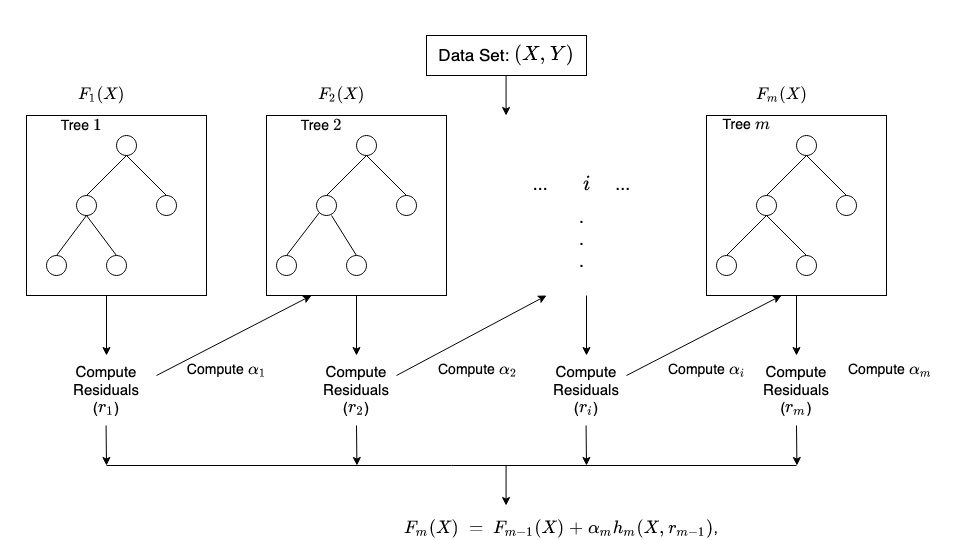
\includegraphics[width=0.9\linewidth]{Images/XGBoost}
	\caption{A concise illustration of how Gradient Boosted Trees work.}
	\label{fig:xgboost}
\end{figure}


\section{Neural Networks}
Artificial Neural Networks (ANNs) are computational models that draw inspiration from the interconnected structure of the human brain. Each individual computational unit, often referred to as an "artificial neuron" or simply "neuron", is designed to mimic the fundamental working mechanism of a biological neuron.

Let's denote the inputs to an artificial neuron as $ x = [x_1, x_2, ..., x_n] $, a representation analogous to dendrites in a biological neuron. These inputs are linearly transformed by a set of weights, $ w = [w_1, w_2, ..., w_n] $, summed together, and a bias term, $ b $, is added to the result. This operation can be expressed mathematically as:

\[
z = \sum_{i=1}^{n} w_i x_i + b 
\]

The calculated value, $ z $, is then passed through an activation function, $ f $, to generate the neuron's output, $ a $. This process can be viewed as the equivalent of the activation potential and the subsequent firing (or not firing) in a biological neuron. The mathematical representation is as follows:

\[
a = f(z)
\]



%TODO: Migliorare la qualità dell imagine, eliminare la parte scritta
\begin{figure}[h!]
	\centering
	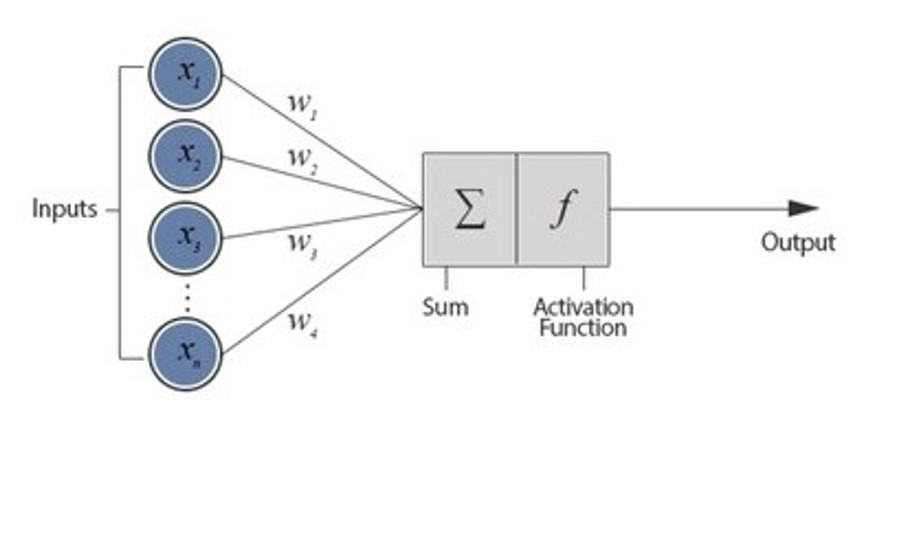
\includegraphics[width=0.8\linewidth]{Images/nn_neuron}
	\caption{}
	\label{fig:nn_neuron}
\end{figure}

The activation function introduces non-linearity into the model, which is crucial for the network's ability to learn complex patterns. Common choices for $ f $ include the sigmoid, hyperbolic tangent, and ReLU (Rectified Linear Unit) functions.\\

An Artificial Neural Network builds upon the concept of the artificial neuron to form an interconnected assembly of these neurons, structured in layers. An ANN typically comprises an input layer, one or more hidden layers, and an output layer. Each layer may contain one or more neurons, and the layers are fully connected, meaning every neuron in one layer connects with all neurons in the following layer.

Follows a grafic rapresentation of a ANN:
\begin{figure}[h!]
	\centering
	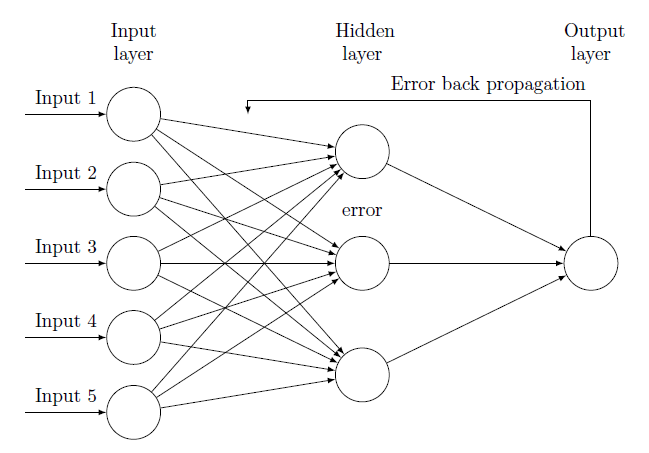
\includegraphics[width=0.7\linewidth]{Images/fig_neural_network}
	\caption{}
	\label{fig:Fig_nn}
\end{figure}


For classification problems, the output layer typically uses a softmax function for multi-class problems to output a probability distribution over the classes, or a sigmoid function for binary classification problems to provide the probability of the positive class.

Training a neural network involves a two-step process: forward propagation and backpropagation. In forward propagation, the input is passed through the network to generate an output. This output is then compared with the actual target to compute the loss function $ L $.

Backpropagation uses the chain rule of calculus to compute the gradient of $ L $ with respect to the network's parameters, which are then used to update the weights and biases:

\[
\frac{\partial L}{\partial w} = \frac{\partial L}{\partial a} \frac{\partial a}{\partial z} \frac{\partial z}{\partial w}
\]

Here, $ \frac{\partial L}{\partial a} $ is the derivative of the loss function with respect to the activation output, $ \frac{\partial a}{\partial z} $ is the derivative of the activation function, and $ \frac{\partial z}{\partial w} $ is the derivative of the weighted sum with respect to the weights.

Once these gradients are calculated, they are used to update the weights and biases via gradient descent, a process that iteratively adjusts the parameters to minimize the loss function:

\[
w_{\text{new}} = w_{\text{old}} - \alpha \frac{\partial L}{\partial w}
\]

\[
b_{\text{new}} = b_{\text{old}} - \alpha \frac{\partial L}{\partial b}
\]

In these equations, $ \alpha $ is the learning rate, a hyperparameter that determines the size of the steps the algorithm takes down the gradient towards the minimum.

The interconnected structure of ANNs, combined with the ability of backpropagation and gradient descent to effectively adjust the model parameters, allows these networks to learn and represent complex, non-linear relationships in the data.
